%!TEX root = ../../statemachineprojekt_entwurf.tex

\newpage
\section{Roboter}
\label{sec:roboter}

\begin{figure}
	\centering
	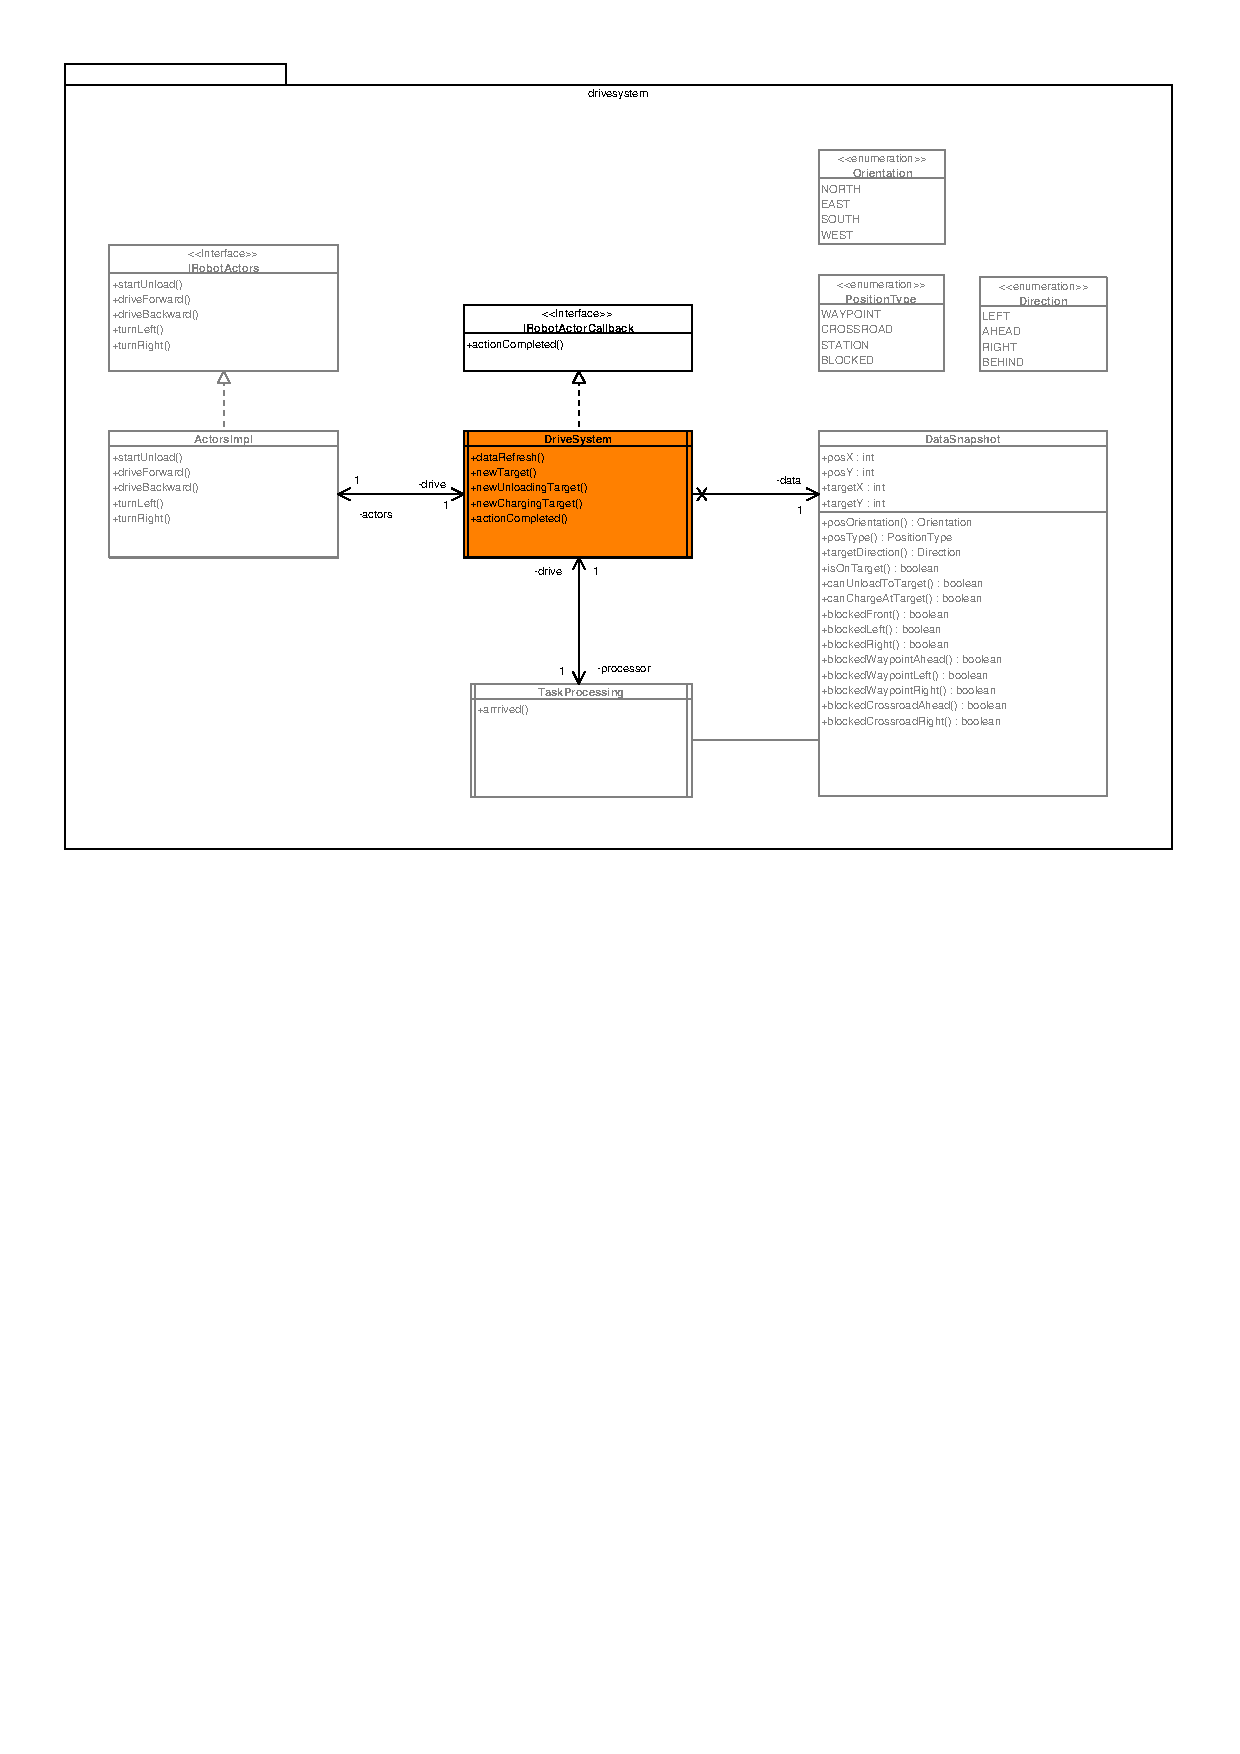
\includegraphics[width=1\textwidth]{robot_classes}
	\caption{UML Klassendiagramm mit einer Auswahl an relevanten Klassen für die Roboter-Software. Die beiden rot markierten aktiven Klassen soll als Zustandsdiagramm umgesetzt werden. Die rot markierte Aufzählung ist mit Inhalten zu füllen.}
	\label{fig:robot_classes}
\end{figure}

Auf allen Robotern laufen die gleichen beiden Ausführungskontexte: Einer zum Abwickeln der Fahr- oder Entladeaufträge (das Ausführungsobjekt ist eine Instanz von \texttt{TaskProcessing}) und einer zum Regeln der Fahraktivitäten selbst (Instanz von \texttt{DriveSystem}). Beide Ausführungskontexte werden beim Systemstart mitgestartet.
Die Klassen sind in \autoref{fig:robot_classes} dargestellt und werden im folgenden genauer beschrieben.



{\color{hpired} \textbf{Hinweis:} In den Unterabschnitten \ref{subsec:robot_task} und \ref{subsec:robot_drive} werden die Klassen beschrieben, welche als Zustandsdiagramm umgesetzt werden sollen. Die übrigen Unterabschnitte liefern Informationen zu den Schnittstellen, die teilweise notwendig zur Umsetzung der Aufgabe sind.}






\subsection{Auftragsabwicklung in \texttt{TaskProcessing}}
\label{subsec:robot_task}

Der Ausführungskontext der Instanz von \texttt{TaskProcessing} dient zur Abwicklung der Aufträge. Er wandelt die eingehenden Nachrichten in Zielvorgaben für die entsprechende Instanz von \texttt{DriveSystem} um.
Wenn der Roboter die Aufgaben erledigt hat, meldet die \texttt{TaskProcessing}-Instanz dies dem Server. 

Getriggert wird die TaskProcessing-Instanz dadurch, dass sie \texttt{IRobotOpFromRemote} implementiert und Aufrufe der Methode \texttt{receive(...)} erhält. Über den Parameter \texttt{function} wird dabei ein Kommando signalisiert, dass in entsprechende Aktivitäten umgesetzt werden muss.
Dazu gehören das Fahren zu einem Abwurfschacht inklusive Entladung sowie die Fahrt zur den einzelnen Positionen einer Abfertigungsstation. Die Rückmeldungen werden durch das Interface \texttt{IRobotOpRemoteCall}, welches über das Attribut \texttt{server} verfügbar ist, umgesetzt. 

Die eigentliche Umsetzung der Fahr- und Entladeaufträge wird an den Ausführungskontext der Instanz von \texttt{DriveSystem} delegiert, die über das Attribut \texttt{drive} erreichbar ist und mit \texttt{stop()}, \texttt{unload()} und \texttt{driveTo(...)} angesteuert wird.
Es Aufgabe von \texttt{TaskProcessing}, die Anweisungen des Servers auf folgen von diesen beiden Befehlen zu reduzieren.
Die \texttt{TaskProcessing}-Instanz empfängt mit den Methoden \texttt{arrived()} bzw. \texttt{unloaded()} asynchrone Rückmeldungen über das erfolgreiche Ankommen oder Abladen.

Zusätzlich nimmt \texttt{TaskProcessing} noch \texttt{batteryEvent()}-Meldungen der Batterie entgegen (siehe \autoref{subsec:robot_battery}), die eventuell an den Server übermittelt werden müssen. Dazu stehen die beiden vordefinierten Konstanten \texttt{BATTERY\_FULL} und \texttt{BATTERY\_LOW} zur Verfügung. Sie definieren, ab welchem oberen Schwellenwert eine Batterie als voll zählt und ab welchem unteren Grenzwert eine Aufladung angefragt werden muss. \texttt{BATTERY\_LOW} ist dabei so gewählt, dass eine Fahrt zur Abfertigungsstation in jedem Fall möglich ist. 






\subsection{Steuerung der Sensoren und Aktuatoren in \texttt{DriveSystem}}
\label{subsec:robot_drive}

Der Ausführungskontext \texttt{DriveSystem} erhält von \texttt{TaskProcessing} Befehle, die umgesetzt werden müssen.
Dazu bietet \texttt{DriveSystem} die Methoden \texttt{stop()}, \texttt{unload()} und \texttt{driveTo(...)} an, entsprechend den drei verschiedene Arten von auszuführenden Aufgaben: Stehenbleiben, die Ladung Abwerfen und zu einer Position Fahren.

Zusätzlich erhält die \texttt{DriveSystem}-Instanz regelmäßige Meldungen des Sensors über die Methode \texttt{sensorEvent(...)} (siehe \autoref{subsec:sensor}) sowie \texttt{unloaded()}-Rückmeldungen der Aktuatoren (siehe \autoref{subsec:actors}).
Zur Interpretation von \texttt{sensorEvent(...)} stehen die privaten Hilfsmethoden \texttt{targetReached(...)} und \texttt{targetDirection(...)} zur Verfügung. Die Menge der Hilfsmethoden kann später noch erweitert werden.


\paragraph{Stehenbleiben}
Während der Roboter steht, wartet er darauf, eine der beiden anderen Aufgaben zu erledigen und ignoriert den Sensortrigger. 


\paragraph{Abladen}
Die Position für das Abladen ist (wie ihn \autoref{sec:umgebung} beschreiben) immer oberhalb des Schachtes. Allerdings kann nur zur (in Fahrtrichtung) rechten Seite hin abgeladen werden. 
Wird der Roboter zum Abladen veranlasst muss also zuerst die Ausrichtung mit aktuellen Sensordaten überprüft und eventuell eine Drehung ausgelöst werden. 
Das Entladen selbst wird dann über die Methode \emph{unload} aus \texttt{IRobotActors} umgesetzt.
Wenn der Vorgang abgeschlossen ist, wird dies dem Attribut \texttt{processor} mit der Methode \texttt{unloaded()} gemeldet und in den stehenden Zustand gewechselt.
Beim Abladen wird der Sensortrigger ignoriert.


\paragraph{Zielanfahrt}
Lautet der Auftrag ein Ziel anzufahren, so wertet der Roboter das periodisch auftretende Ereignis vom Sensor aus, indem er auf den Trigger \texttt{sensorEvent(...)} reagiert (siehe \autoref{subsec:sensor}). 

Im Bereich der \textbf{Abfertigungsstationen} wird für alle kritischen Stellen serverseitig eine exklusive Fahrfreigabe eingeholt, sodass Kollisionen bei den Batterieaufladepositionen ausgeschlossen sind. Durch die Trennwände ist die jeweilige Fahrspur stark eingeschränkt, was die Fahrstrecke bestimmt.
Da die Warteschlange Teil der Station ist und nicht von der Exklusivfreigabe abgedeckt wird, muss vor dem Vorwärtsfahren immer geprüft werden, dass das direkt voraus liegende Feld tatsächlich frei ist.

Im eigentlichen \textbf{Sortierbereich} werden Kollisionen durch das in \autoref{sec:umgebung} beschriebene \emph{Rechtsfahrgebot} in Kombination mit einer \emph{Rechts vor Links Vorfahrtsregel} ausgeschlossen. 
Das Fahrverhalten besteht dabei aus drei möglichen Aktivitäten (siehe \autoref{fig:move}):
\begin{enumerate}
	\setlength\topsep{-1em}
	\setlength\itemsep{-0.5em}
	\item \label{step1} Die Fahrt von einem Wegpunkt auf die Ecke einer Kreuzung, wobei beachtet werden muss, dass die Kreuzung frei ist und niemand gemäß Rechts vor Links Vorfahrt hat.
	\item \label{step2} Der Richtungswechsel (und damit verbunden ein Wechsel der Fahrspur) von einem Wegpunkt aus, was z.B. für das Erreichen der Entladeposition nötig sein kann.
	\item \label{step3} Das Verlassen einer Kreuzung zum nächsten Wegpunkt, wobei der Roboter sich für einen von drei Richtungen (Wegpunkten) entscheiden kann (und der entsprechende Wegpunkt frei sein muss). Die Fahrt vom ersten befahrenen Punkt der Kreuzung bis zum Wegpunkt kann in einem Zug erfolgen.
\end{enumerate}


\begin{figure}[t]
	\centering
	\begin{subfigure}[b]{0.45\textwidth}
		\centering
		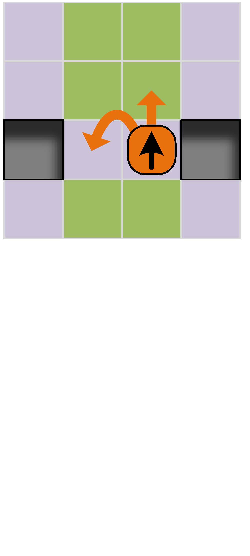
\includegraphics[scale=0.9]{robot_move_1}
		\caption{Vom Wegpunkt aus: Wenden oder geradeaus auf das erste Feld der Kreuzung fahren.}
		\label{fig:move_1}
	\end{subfigure}
	~~~~~
	\begin{subfigure}[b]{0.45\textwidth}
		\centering
		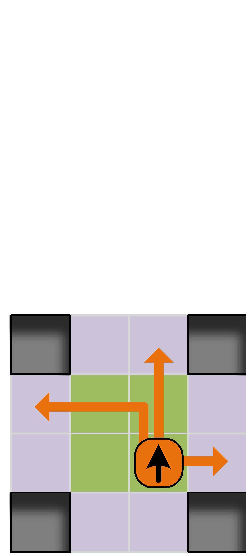
\includegraphics[scale=0.9]{robot_move_2}
		\caption{Von einer Kreuzung aus: Verlassen der Kreuzung in drei verschiedene Richtung.}
		\label{fig:move_2}
	\end{subfigure}
	\caption{Mögliche Fahraktivitäten im Sortierbereich, abhängig von der aktuellen Postion.}
	\label{fig:move}
\end{figure}

Die Fahrten folgen dem folgenden Muster: Es wird zuerst nach Norden, dann nach Westen oder Osten und erst ganz zuletzt in südliche Richtung gefahren. Auf dem Weg zu einer Abladeposition wird so zuerst von der Abfertigungsstationen aus geradeaus nach Norden bis auf die richtige Höhe gefahren, danach zur Seite und danach ggf (durch eine Fahrt um ein Feld nach Süden) die Richtung gewechselt). Auf dem Rückweg entfällt eine Fahrt nach Norden, es wird also zuerst die richtige Ost-West-Ausrichtung angepeilt und dann geradeaus nach Süden fahren zu können.
Aus Sicht des lokalen Roboters übersetzt sich das in die Regel: Erst geradeaus und möglichst spät abbiegen.

Hat ein Roboter seine Zielposition erreicht meldet er es über die Methode \texttt{arrived} am Attribut \texttt{processor} und wechselt in den stehenden Zustand.






\subsection{Sensorergebnisse mit \texttt{ISensorInfo}}
\label{subsec:sensor}


Die Sensoren senden in regelmäßigen Abständen ein \texttt{sensorEvent(...)} an \texttt{ISensorInfo}. Wenn die \texttt{DriveSystem}-Instanz das \texttt{sensorEvent(...)} nicht direkt bearbeiten kann verfällt die Eingabe.

\texttt{sensorEvent(...)} liefert Objekte der Klasse \texttt{SensorData}. Die \texttt{SensorData}-Objekte beinhalten die eigentlichen Daten in Form von \texttt{RawSensorData}. Verwendbare Informationen können mittels gegebener Zugriffsmethoden abgefragt werden:
\begin{itemize}
	\setlength\topsep{-1em}
	\setlength\itemsep{-0.5em}
 	\item \texttt{pos()} liefert die aktuelle Position durch.
 	\item \texttt{posType()} gibt an, auf welcher Art von Position er sich befindet (\texttt{CROSSROADS}, \texttt{WAYPOINT} oder \texttt{STATION}).
 	\item \texttt{posOrientation()} bestimmt, in welcher Himmelsrichtung der Roboter orientiert ist.
 	\item \texttt{blockedFront()}, \texttt{blockedLeft()} und \texttt{blockedRight()} zeigen, ob die benachbarten Positionen durch einen Roboter oder ein Hindernis blockiert sind oder hinter einer Trennwand liegen (siehe auch \autoref{fig:sensor_1}). Ein Feld zählt als blockiert, wenn auch nur kleinste Teile davon belegt sind (z.B. durch das vorderste Stück eines einfahrenden Roboters).
\end{itemize}

\begin{figure}[t]
	\centering
	\begin{subfigure}[b]{0.45\textwidth}
		\centering
		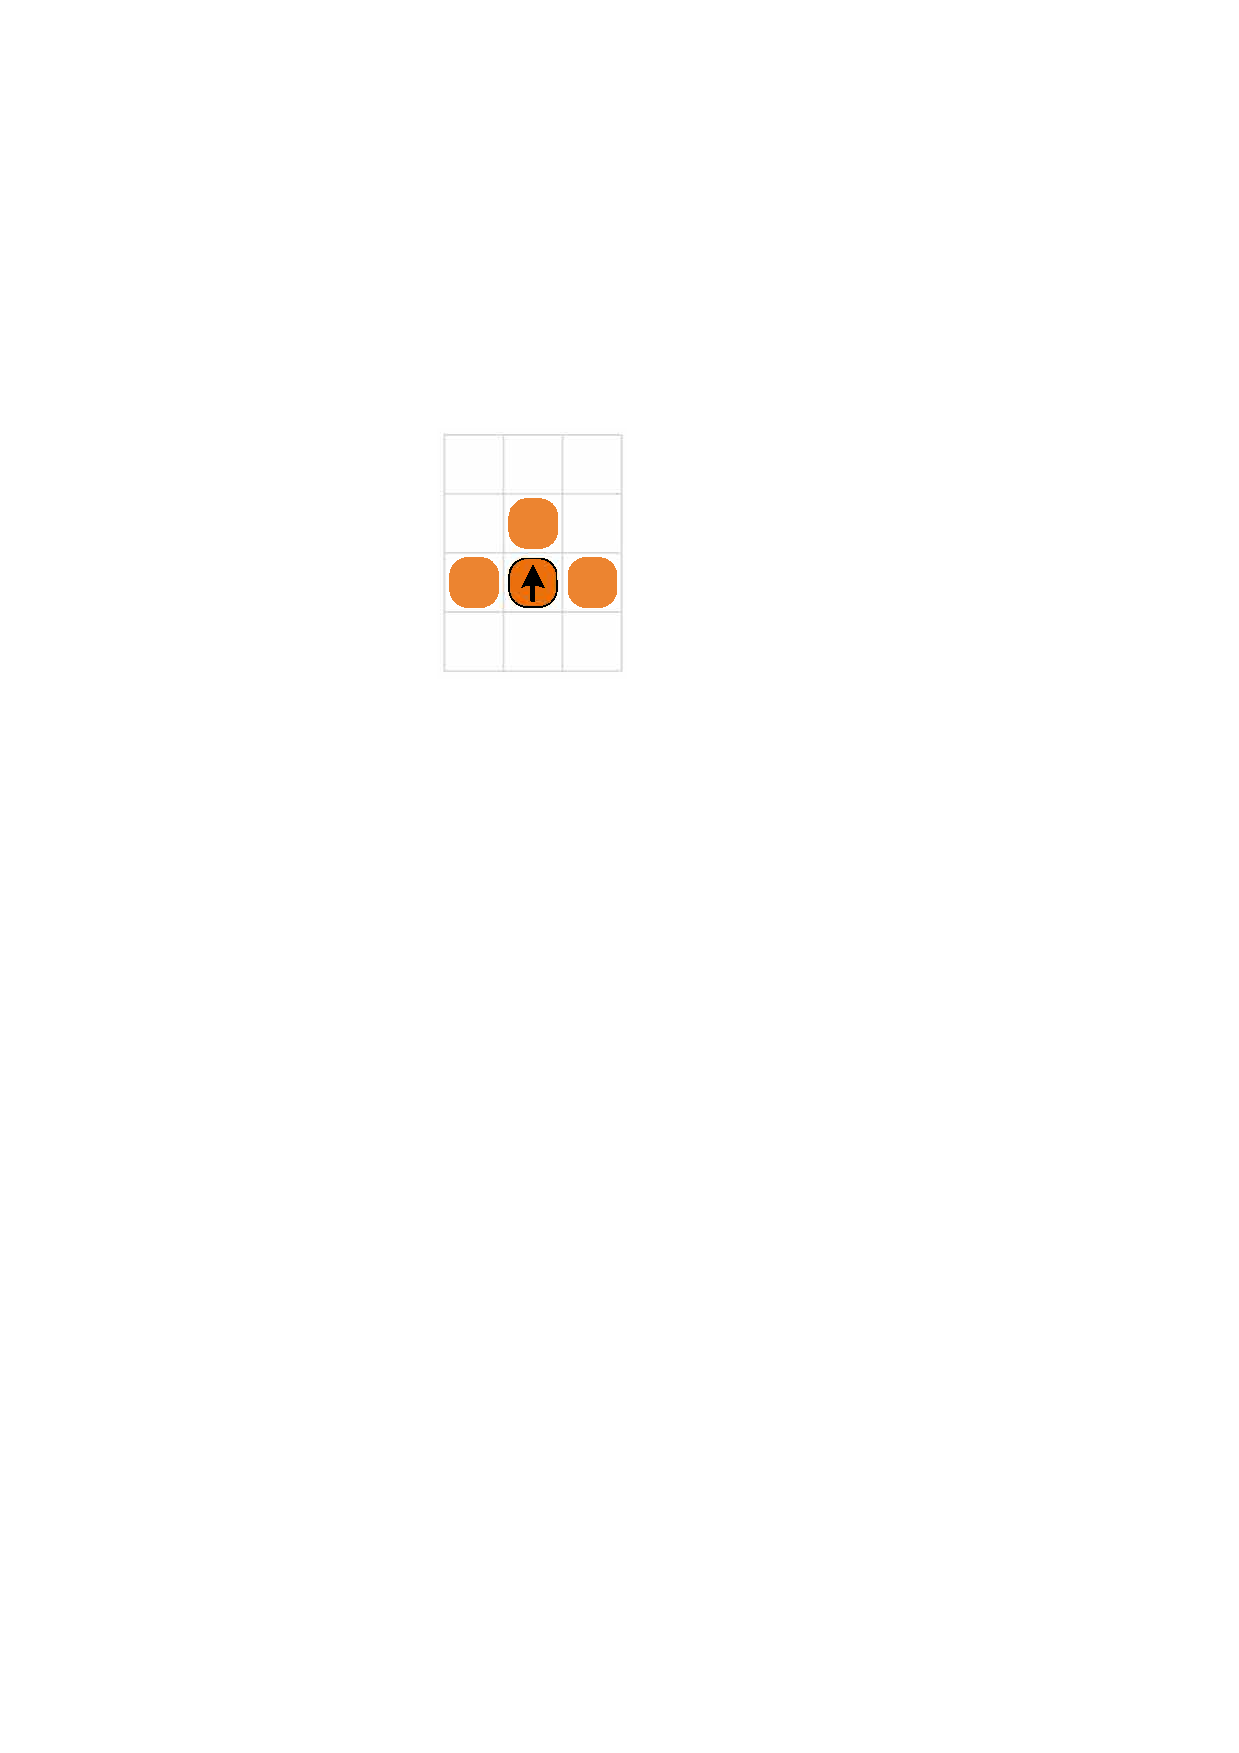
\includegraphics[scale=0.9]{sensor_1}
		\caption{Hindernisabfrage der direkt benachbarten Felder mit \texttt{blockedFront()}, \texttt{blockedLeft()} und \texttt{blockedRight()}. Trennwände zählen wie Hindernisse.}
		\label{fig:sensor_1}
	\end{subfigure}
	~~~~~
	\begin{subfigure}[b]{0.45\textwidth}
		\centering
		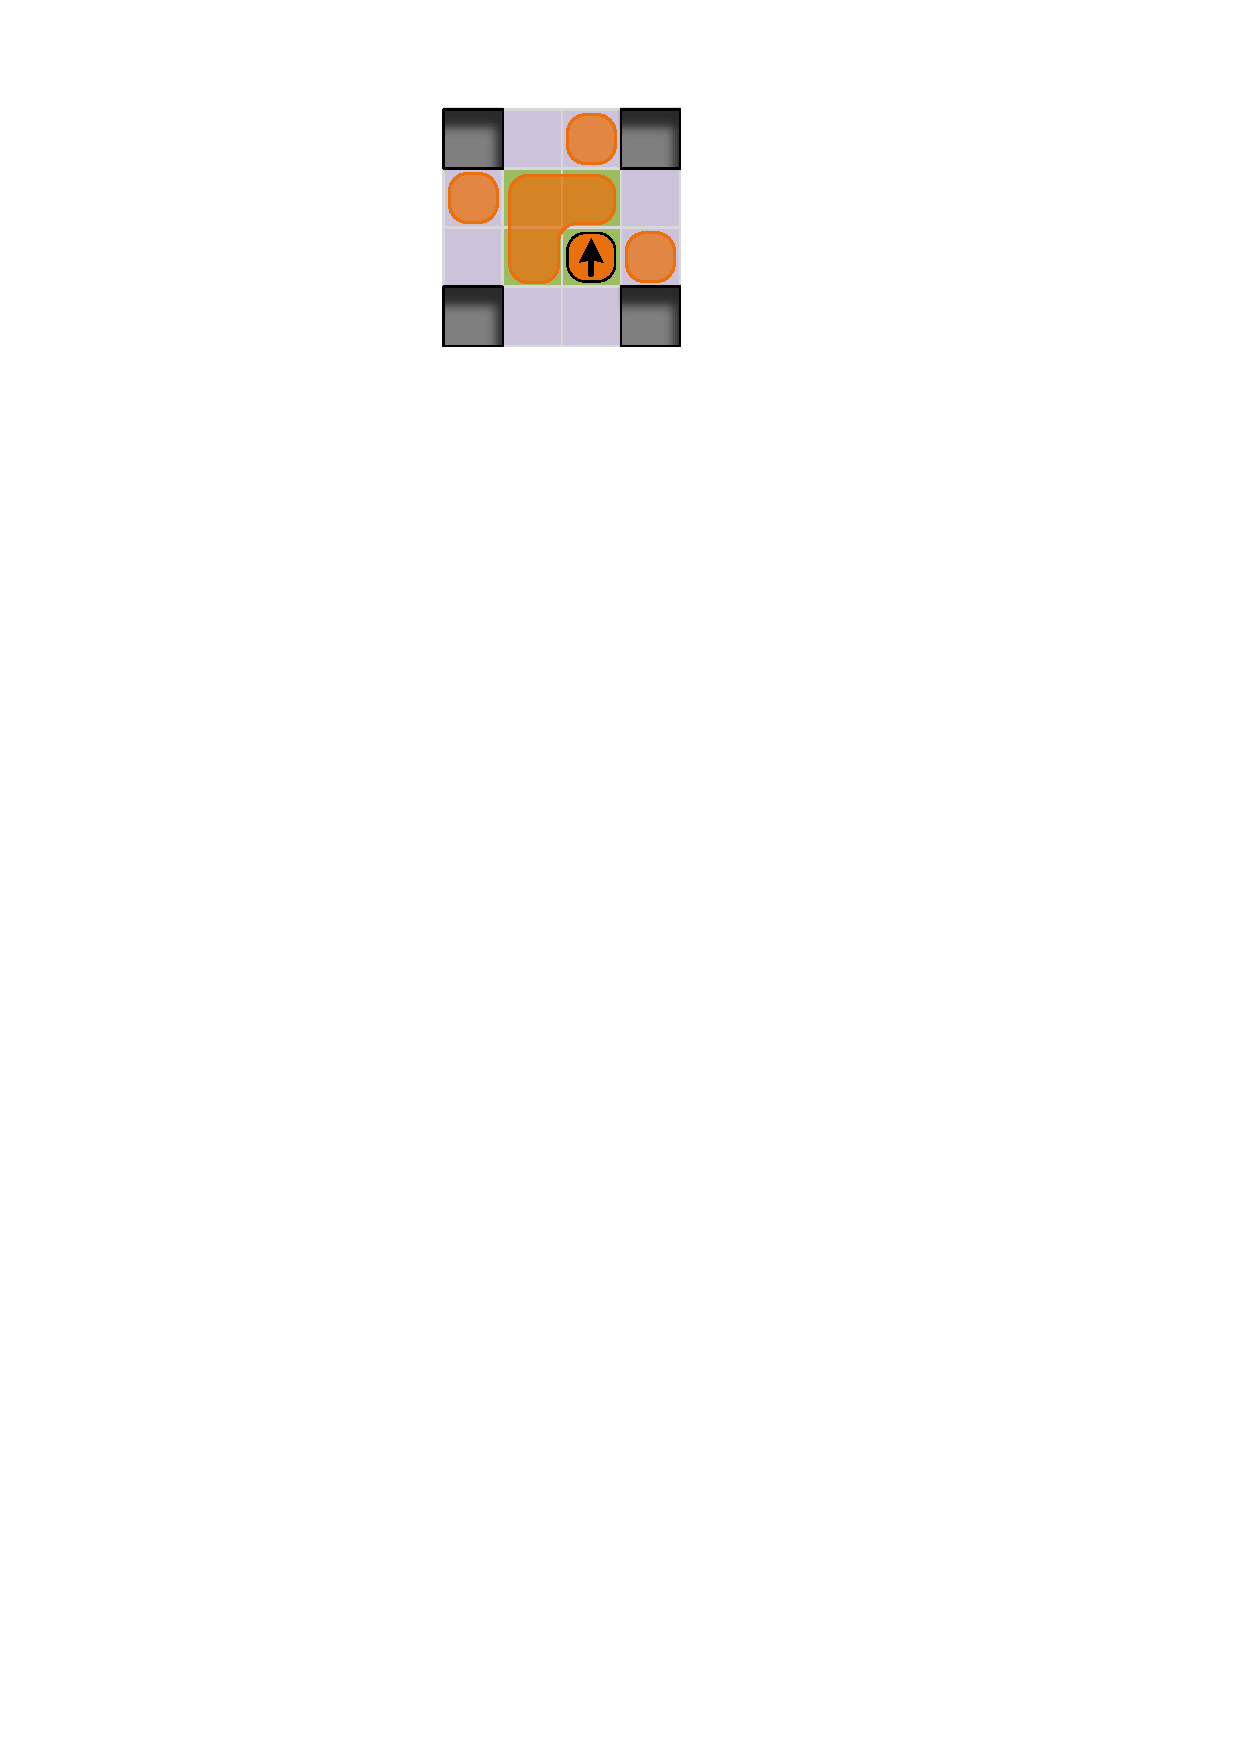
\includegraphics[scale=0.9]{sensor_2}
		\caption{Hindernisabfrage der benachbarten Wegpunkte mit \texttt{blockedWaypoint*()} und \texttt{blockedCrossroadAhead()}, ausgehend vom ersten Feld einer Kreuzung.}
		\label{fig:sensor_2}
	\end{subfigure}
	\begin{subfigure}[b]{0.45\textwidth}
		\centering
		\vspace{1cm}
		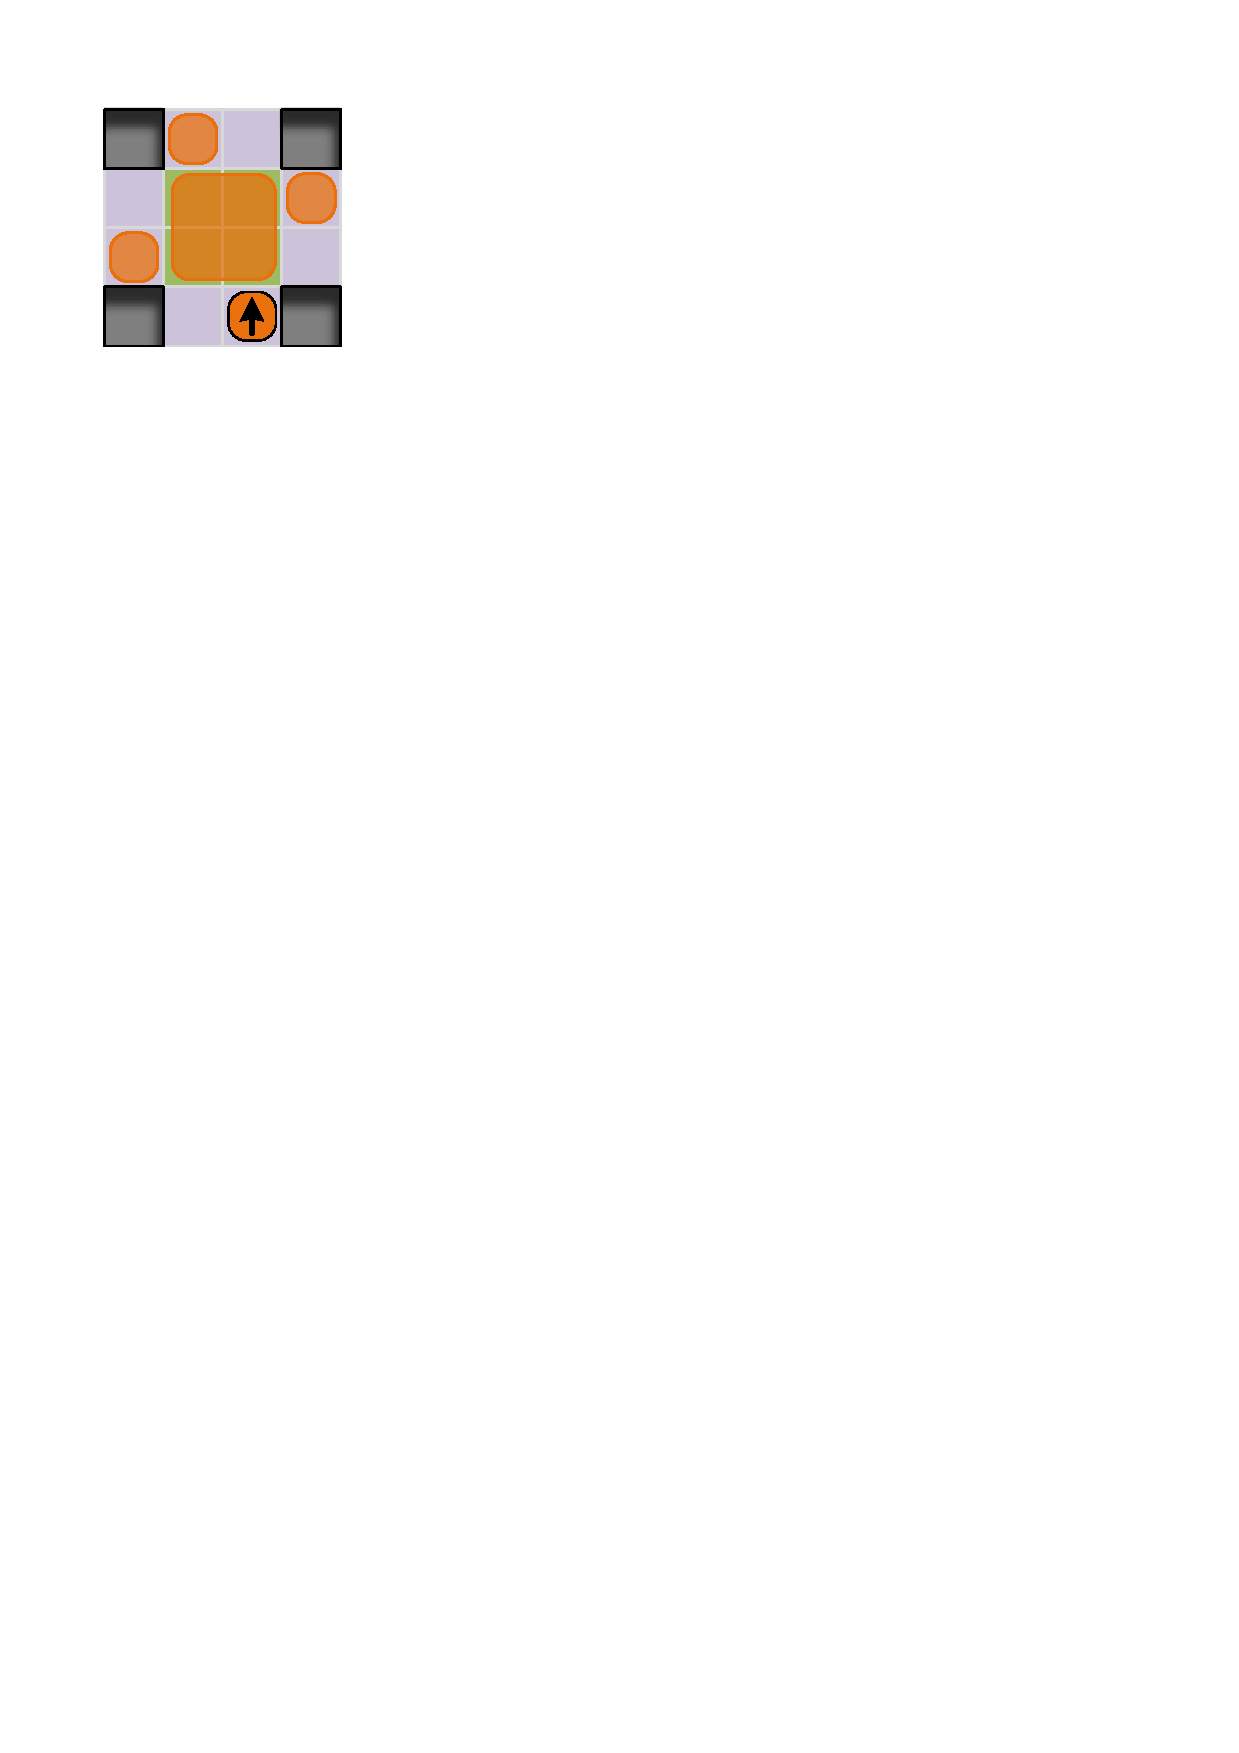
\includegraphics[scale=0.9]{sensor_3}
		\caption{Hindernisabfrage für eine voraus liegende Kreuzung sowie die dahinter liegenden Wegpunkte mit \texttt{blockedCrossroadAhead()} sowie \texttt{blockedWaypoint*()}, wenn der Roboter selbst auf einem Wegpunkt steht.}
		\label{fig:sensor_3}
	\end{subfigure}
	~~~~~
	\begin{subfigure}[b]{0.45\textwidth}
		\centering
		\vspace{1cm}
		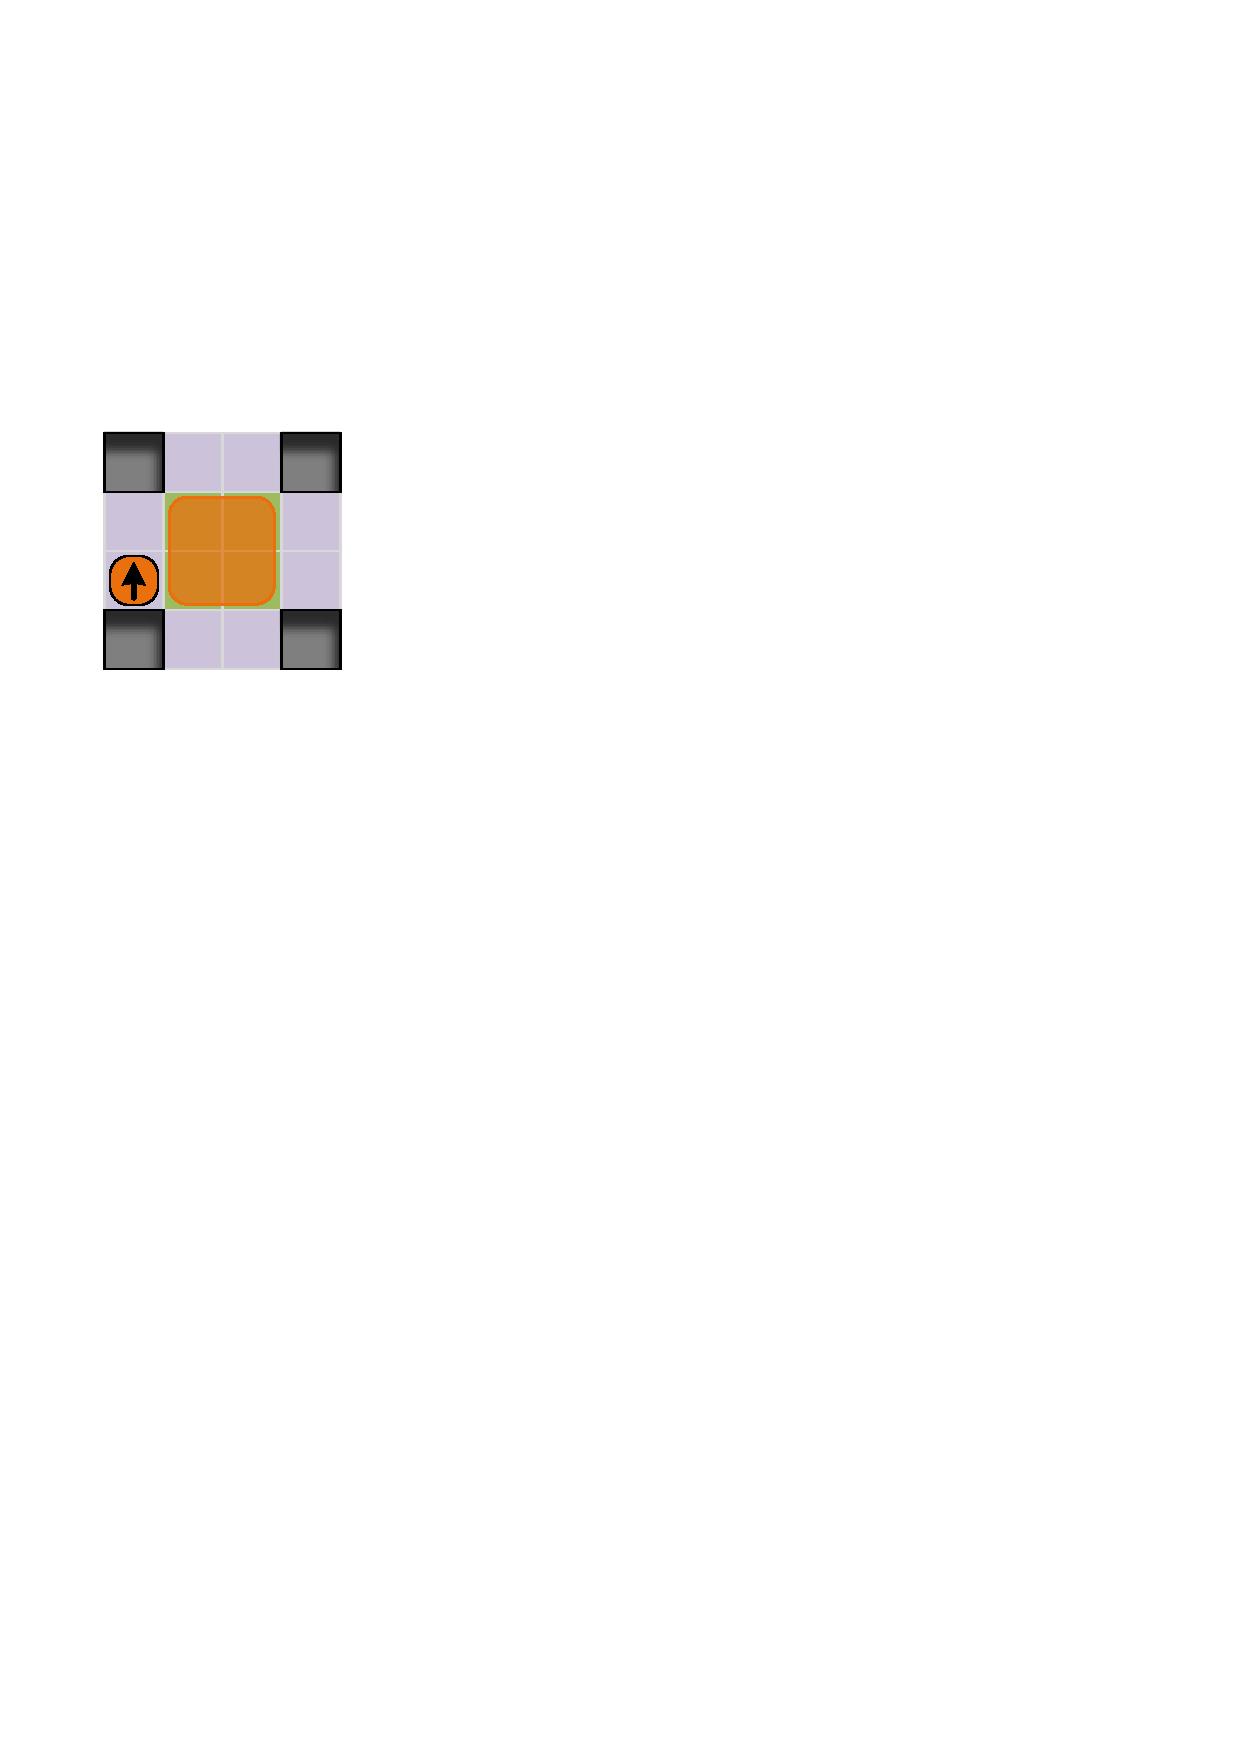
\includegraphics[scale=0.9]{sensor_4}
		\caption{Hindernisabfrage für eine rechts liegende Kreuzung mit \texttt{blockedCrossroadRight()}. Ist diese Kreuzung leer kann garantiert werden, dass kein anderer Roboter das voraus liegende Feld erreichen kann.}
		\label{fig:sensor_4}
		\vfill{}
	\end{subfigure}
	\caption{Funktionsweise der (teilweise kontextsensitiven) \texttt{blocked*()}-Methoden, mit denen ein Roboter prüft ob Felder in der Umgebung blockiert sind.}
	\label{fig:sensor}
\end{figure}


\paragraph{Abfrage von Kreuzungen und Wegpunkten}
Zusätzlich gibt es weitere Zugriffsmethoden, die speziell auf den Verkehr in der Sortieranlage ausgelegt sind und gezielt überprüfen, ob Kreuzungen und Wegpunkten von einem anderen Roboter blockiert werden. In \autoref{fig:sensor} ist die designierte Nutzung von \texttt{blockedWaypoint*()} und \texttt{blockedCrossroad*()} visualisiert.

Mit \texttt{blockedCrossroadAhead()} wird die voraus liegende Kreuzung überprüft (siehe \autoref{fig:sensor_3}) \emph{oder} der \enquote{Rest} der aktuell selbst befahrenen Kreuzung (siehe \autoref{fig:sensor_2}). Mit \texttt{blockedCrossroadRight()} (siehe \autoref{fig:sensor_4}) die Kreuzung zu rechten des Roboters überprüft. Letztere Überprüfung ist relevant, wenn der Roboter die Spur wechseln will.

Wegpunkte werden mittels den drei \texttt{blockedWaypoint*()}-Methoden überprüft.
Wenn der Roboter sich dabei selbst auf einem Wegpunkt mit Blick auf eine Kreuzung befindet befindet, werden die Wegpunkt-Positionen erfasst, die ebenfalls auf die Kreuzung einfahren könnten (siehe \autoref{fig:sensor_3}). Befindet er sich auf einer Kreuzung, werden die abgehenden Wegpunkte erfasst, die der Roboter nach verlassen der Kreuzung erreichen würde (siehe \autoref{fig:sensor_2}).

Sämtliche \texttt{blockedWaypoint*()} und \texttt{blockedCrossroad*()}-Methoden agieren dabei nach dem Prinzip \enquote{garbage in, garbage out}, wenn sie außerhalb der designierten Positionen genutzt werden. So ist z.B. undefiniert, welche Antwort \texttt{blockedCrossroadAhead()} in einem Stationsbereich liefert.







\subsection{Zugriff auf die Aktuatoren mit \texttt{IRobotActors} und \texttt{IRobotActorInfo}}
\label{subsec:actors}

Die über die Schnittstelle \texttt{IRobotActors} ansteuerbaren Aktuatoren teilen sich in zwei Gruppen ein.

Auf der einen Seite gibt es die atomaren Fahrbefehle \texttt{driveForward()}, \texttt{turnLeft()} und \texttt{turnRight()}. Dabei bewegt sich \texttt{driveForward()} immer strikt ein Feld im Koordinatensystem vorwärts (siehe \autoref{sec:umgebung}).
Bei den Fahrbefehlen handelt es sich um \emph{synchrone} Aufrufe, das heißt der Aufruf ist erst dann beendet, wenn der Fahrbefehl ausgeführt worden.

Auf der anderen Seite bietet \texttt{IRobotActors} den \emph{asynchronen} Aufruf \texttt{unload()}, welcher den Entladeprozess auslöst. Beim Endladen wird die Roboter-Beladung immer zur (in Fahrtrichtung) rechten Seite hin abgeworfen.
Als Rückmeldung bei beenden des Abladens wird über \texttt{IRobotActorInfo} automatisch die Methode \texttt{unloaded()} aufgerufen.





\subsection{Batteriestandkontrolle mit \texttt{IBatteryInfo}}
\label{subsec:robot_battery}

Die Batteriesteuerung sendet regelmäßig \texttt{batteryEvent(...)} Trigger an den Ausführungskontext der \texttt{TaskProcessing} Instanz, welche das Interface \texttt{IBatteryInfo} implementiert. 
Die \texttt{batteryEvent(...)} Meldung erhält einen Fließkommawert zwischen 0 und 1, der mit entsprechenden Schwellenwerten verglichen werden kann. 



\subsection{Kommunikation über \texttt{IRobotOpRemoteCall} und \texttt{IRobotOpFromRemote}}

Zur Kommunikation stellt \texttt{RobotCommunication} die Schnittstellen \texttt{IRobotOpRemoteCall} und \texttt{IRobotOpFromRemote} zur Verfügung.

Analog zu \texttt{IServerOpRemoteCall} bietet \texttt{IRobotOpRemoteCall} eine Methode \texttt{send(...)}, welche allerdings keine \texttt{id} benötigt, da immer der gleiche fest einprogrammierte Server angesprochen wird. 
Es wird ein Literal aus \texttt{Notification} ohne Positionsangabe versendet.

Auf der Gegenseite können über \texttt{receive(...)} an der Schnittstelle \texttt{IRobotOpFromRemote} an den Roboter gerichtete Nachrichten zugestellt werden. Die Nachrichten bestehen aus einem \texttt{Command}-Literal und einer (optionalen) \texttt{Position}.